\documentclass[prodmode,acmtap]{acmlarge}

\usepackage[utf8x]{inputenc}
\usepackage[italian]{babel}
\usepackage{epstopdf}
\usepackage{graphicx}
\usepackage[hang,small,bf]{caption}
\usepackage{babel,blindtext}
%\usepackage{subcaption}



% Metadata Information
\acmVolume{1}
\acmNumber{1}
\acmArticle{1}
\articleSeq{1}
\acmYear{2013}
\acmMonth{6}

% Package to generate and customize Algorithm as per ACM style
\usepackage[ruled]{algorithm2e}
\SetAlFnt{\algofont}
\SetAlCapFnt{\algofont}
\SetAlCapNameFnt{\algofont}
\SetAlCapHSkip{0pt}
\IncMargin{-\parindent}
\renewcommand{\algorithmcfname}{ALGORITHM}


% Title portion
\title{Analisi della stabilità del protocollo di DHT Symphony\\
\Large{Relazione sul Progetto di Simulazione di Sistemi}
}
\author{MATTEO BRUCATO e MIRO MANNINO\affil{Università di Bologna}
}


\begin{abstract}
Symphony è un protocollo di overlay per sistemi peer-to-peer in grado di mantenere una tabella hash distribuita (DHT) attraverso nodi che risiedono in una rete geografica.
\vspace*{50mm}
\end{abstract}

\category{}{}{}[]


\begin{document}

\maketitle


\section{Introduzione}
% Cos'è Sympony e cosa vogliamo verificare con la simulazione (stabilità, perché?)

Symphony~\cite{symphony} è un protocollo per tabelle hash distribuite (DHT) che, attraverso una rete di overlay costruita in base a particolari distribuzioni armoniche, è in grado di garantire lookup efficienti, poli-logaritmici nel numero di hop (salti), ovvero nella sua \emph{latenza}\footnote{In sintonia con la terminologia tipica della letteratura peer-to-peer, indichiamo col termine \emph{latenza} il numero medio di hop per l'operazione di lookup.}.

Attraverso un concetto denominato \emph{greedy routing}, è stato mostrato come sia possibile indirizzare e consegnare un messaggio ad un qualsiasi nodo in una rete in al più $O(log^2 n)$ salti (un fenomeno chiamato anche \emph{Small World})~\cite{small-world}. Symphony si basa esattamente su questi concetti, i quali vengono applicati magistralmente al caso di reti peer-to-peer e al problema di creare DHT. In particolare, Symphony è in grado di garantire una latenza di $O(\frac{1}{k} log^2 n)$ salti, dove $k=O(1)$ è il numero di link che ogni nodo mantiene verso altri nodi della rete.

Nell'articolo in cui Symphony è stato presentato~\cite{symphony}, vengono evidenziati i molteplici vantaggi del protocollo rispetto ai suoi predecessori (Chord, Viceroy, ecc.). Il vantaggio più evidente è quello di richiedere un numero costante $k=O(1)$ di link verso altri nodi della rete, a differenza di protocolli come Chord~\cite{chord} che richiedono un numero logaritmico di link uscenti.

Symphony, inoltre, è dimostrato essere \emph{scalabile} nella dimensione della rete, ..................

Infine, gli autori dichiarano anche il sistema \emph{stabile}, ovvero capace di funzionare nel caso in cui gli host si uniscano alla rete ed escano dalla rete in maniera del tutto arbitraria, tipicamente con brevi periodi di vita. Ciononostante, un'approfondita analisi dell'articolo mostra come gli esperimenti effettuati per stabilire la stabilità di Symphony offrano solamente una panoramica limitata sui possibili scenari che possano veramente essere fonte di instabilità. I test effettuati non sono tali da stressare il sistema fino ai punti più critici, in cui un'evidente instabilità possa essere misurata.

Lo scopo del presente elaborato è quello di studiare a fondo la stabilità del protocollo Symphony, e di stabilire in maniera più accurata se tale protocollo può essere veramente considerato stabile e in che misura. Più precisamente, ci poniamo l'obiettivo di valutare la stabilità del protocollo sotto carichi di stress causati da \emph{churn}, ovvero da alte frequenze di entrata e uscita dei nodi della rete. Studieremo sotto quali condizioni di stress la stabilità del protocollo vale e in quali condizioni essa comincia a vacillare.

Attraverso una serie di esperimenti in simulazione, mostreremo come il protocollo Symphony risponda molto bene a situazioni di stress causato da \emph{churn} simili a quelle testate dagli autori dei protocollo. E' solo con l'ausilio di un \emph{motore di churn} molto sofisticato che siamo in grado invece di stressare il sistema fino a fargli perdere la sua stabilità. I nostri esperimenti, infatti, mostrano che ..................

La relazione è organizzata nel seguente modo. In Sezione~\ref{symphony} descriveremo brevemente il protocollo Symphpny. In Sezione~\ref{stabilita} descriveremo formalmente il concetto di stabilità che sarà oggetto di valutazione del protocollo in esame. In Sezione~\ref{simulatore}, presenteremo i dettagli sul simulatore realizzato, il livello di astrazione del simulatore stesso e dettagli sulla sua realizzazione. La Sezione~\ref{risultati} raccoglierà i risultati sperimentali delle simulazioni, mentre la Sezione~\ref{conclusioni} illustrerà le nostre conclusioni.





\section{Il protocollo Symphony} \label{symphony}
% Breve introduzione ai termini del paper: join, leave, re-linking, ... tutto quello usato nel resto...
Symphony è un protocollo DHT basato su un'overlay strutturato con topologia ad anello. Gli identificatori dei nodi sono selezionati in maniera randomica uniforme nell'intervallo $[0,1)$. Ogni nodo $p_i$ con identificatore $x$ gestisce il sotto-intervallo dell'anello $(y,x]$ se $y$ è l'identificatore del peer $p_{i-1}$ immediatamente precedente al peer $p_i$. In questo modo ogni valore $x \in [0,1)$ è gestito (univocamente) da uno ed un solo peer, che chiameremo il \emph{manager} di $x$ nel resto della presente relazione.

\subsection{Collegamenti tra nodi}
I nodi della rete Symphony sono collegati tra loro secondo due tipi di link: \emph{short link} e \emph{long link}, ovvero collegamenti a breve e lungo raggio. I collegamenti short servono a creare la struttura ad anello vera e propria: un peer $p_i$ è collegato per mezzo di due short link ai due peer $p_{i-1}$ e $p_{i+1}$ (supponendo sempre aritmetica modulo $n$), ovvero il suo predecessore e il suo successore nell'anello. I collegamenti long, invece, servono a permettere salti a lunga distanza nell'anello, i quali determinano la complessità logaritmica del protocollo di routing di Symphony. I long link sono quindi la caratteristica più importante del protocollo in esame.

Ogni nodo mantiene $k \ge 1$ long link. La scelta dei peer a cui collegarsi è la peculiarità principale del protocollo Symphony. Ogni nodo, quando deve decidere a chi collegarsi per mezzo di un long link, utilizza un numero randomico $x \in [0,1)$ selezionato sulla base di una distribuzione di probabilità appartenente ad una famiglia di distribuzione armoniche, una versione continua della distribuzione discreta di Kleinberg.


\subsection{Join}
Quando un peer vuole entrare nella rete





\section{Analisi della Stabilità} \label{stabilita}
% definizione formale e pochi esempi

Nell'articolo originale~\cite{symphony}, gli autori Manku et al. testano la stabilità del protocollo Symphony in una cosiddetta \emph{rete dinamica}, ovvero una rete in cui i nodi entrano ed escono arbitrariamente. In particolare, gli autori studiano una rete di centomila nodi, ognuno dei quali ha un numero logaritmico di vicini e alterna uno stato di attività ad uno stato di inattività. I tempi di attività e inattività sono tratti da due distribuzioni esponenziali diverse, tali che i nodi restino attivi per poco tempo (in media mezz'ora) e inattivi per il resto della giornata (23 ore e mezza in media). Le distribuzioni esponenziali fanno sì che la stragrande maggioranza dei nodi rispecchino questo comportamento.

Questo setup rispecchia certamente alcuni scenari veritieri di utilizzo dei sistemi DHT. I nodi entrano nella rete una volta al giorno e vi rimangono per pochissimo tempo (forse il tempo necessario per fare una semplice ricerca e scaricare uno o due file). Ciononostante non è certamente atto a coprire la maggioranza dei casi di utilizzo possibili, specialmente quelli in cui la rete venga stressata in maniera molto più pesante. Si pensi ad esempio ad un utilizzo di una DHT da parte di altri sistemi, in sistemi distribuiti integrati fra loro. In tali situazioni, non si può fare nessuna supposizione né sugli orari di utilizzo, né sulla durata d'utilizzo o sulla frequenza di entrata nella rete.

Non solo lo scenario usato nei test dagli autori di Symhony prevede una frequenza di entrata e uscita piuttosto basse, ma gli autori assumono anche una crescita della rete molto controllata. Nei loro test, infatti, essi fanno crescere la rete in maniera lineare durante l'arco di una giornata. Alla fine della prima giornata, tutti i centomila nodi sono entrati nella rete, e vi rimangono durante tutto l'arco della giornata successiva. Durante il terzo giorno, invece, i peer vengono fatti uscire dalla rete a intervalli regolari. Non siamo riusciti ad immaginare, in questo caso, un esempio di utilizzo reale che rispecchi questo particolare test. Ma soprattutto, ancora, questo test non è atto a stressare la rete con un'adeguata frequenza di churn, o in casi di altissima e imprevedibile attività.

Infine, i test riguardanti la stabilità presenti nell'articolo considerano solo reti senza re-linking. Reputiamo molto interessante stabilire cosa accade in una rete sotto churn nel caso in cui il re-linking sia attivo, in quanto esso forza molti peer a distruggere e ricreare tutti i propri long link, i quali sono quelli che contribuiscono maggiormente alle performance del protocollo stesso.


\subsection{Modello di stabilità}

Il modello di stabilità che vogliamo considerare nel presente elaborato è più complesso e a grana più fine di quello utilizzato nel paper originale. Innanzitutto, osserviamo come il tempo di permanenza di un certo peer nella rete è ininfluente rispetto la misura di stabilità della rete. Sapere che un peer sta nella rete per mezz'ora o per un giorno non fa alcuna differenza. Ciò che può maggiormente influire sulla stabilità è il fatto che una grande quantità di peer chiedano un lookup mentre la rete è in fase di creazione a seguito di \emph{join} (entrate) e \emph{leave} (uscite) dei peer.

L'ipotesi alla base dei nostri test è che durante i join (e/o i leave) l'anello di Symphony possa avere potenziali punti di inefficienza dati dal fatto che i peer che stanno entrando non hanno ancora terminato la fase di linking necessaria alla rete per funzionare nei tempi logaritmici. Aumentare il numero di peer che fanno join o leave per istante di tempo dovrebbe quindi evidenziare tale inefficienza nelle misurazioni delle latenze dei lookup.

Ciò che quindi sembra poter avere un impatto più preponderante sulla stabilità non è il tempo di permanenza del singolo peer, ma la \emph{frequenza del fenomeno di churn} (sia esso di leave o di join). Il nostro modello, quindi, prevede di potere valutare la stabilità del sistema al variare della frequenza di join e/o di leave nel sistema.

Questo approccio offre anche numerosi vantaggi in termini di flessibilità nei test. .... [poter concentrarci sulla frequenza di churn ignorando dettagli come tempo di permanenza, orario di entrata e uscita, effettiva grandezza della rete ad ogni istante di tempo permettono di effettuare test di stabilità più generali]


\subsection{Misurare la stabilità}

Una buona rete peer-to-peer senza struttura garantisce in generale che un lookup non richieda un numero di salti maggiore del numero di nodi della rete. Nel caso pessimo, infatti, la rete invia il messaggio di lookup a tutti i peer della rete finché il peer destinatario non viene contattato. L'upper bound del lookup è cioè $O(n)$ per qualunque rete peer-to-peer non banale.

Una rete strutturata come Symphony, in generale, garantisce molto meglio: un upper bound logaritmico nel numero di salti necessari ad un singolo lookup.
Ciononostante, se $n$ peer dovessero entrare tutti contemporaneamente, prima che la rete sia riuscita a creare la struttura necessaria a garantire l'upper bound teorico, le prestazioni potrebbero essere molto peggiori del previsto, fino al caso pessimo di lookup in $O(n)$ salti, come nel caso di rete senza struttura.

Bisogna inoltre considerare che l'upper bound teorico non corrisponde per forza al numero di hop necessari, e può essere anche molto più alto (pessimistico) rispetto a ciò che avviene nella realtà. Una buona struttura e un buon protocollo possono, in media, garantire numero di salti molto minori dell'upper bound teorico.

Ciononostante, è plausibile aspettarsi che uno stress maggiore o minore del sistema possa modificare, in media, il numero effettivo di salti necessari al processamento dei lookup. Ciò potrebbe portare le prestazioni del sistema ad essere nella media più vicine all'upper bound teorico. Nel seguito ci riferiamo a questo trend, se presente e misurabile, come una forma di \emph{instabilità} di un protocollo di lookup. Di contro, un sistema è più stabile tanto più le sue prestazioni rimangono eguali indipendentemente dallo stress momentaneo subito dal sistema, e tanto più il numero di salti dell'algoritmo di lookup misurati sperimentalmente si discosti dall'upper bound teorico. Tale stress è caratterizzato, come detto in precedenza, dalla frequenza di join o di leave dei peer della rete.

Introduciamo quindi, ai fini della nostra analisi, le seguenti definizioni di \emph{stabilità}: (1) la stabilità di un singolo lookup, (2) la stabilità di una serie di misurazioni di lookup, e infine la (3) stabilità di un protocollo di DHT.

\begin{definition}{(\textsc{Stabilità di un lookup})}
Dato un certo protocollo DHT e una misurazione relativa ad un singolo lookup $(h,n)$ dove $h$ è il numero di hop (salti) del lookup e $n$ è il numero di peer presenti nella rete all'istante della terminazione del lookup, la stabilità del lookup è definita come:
$$ s(h,n) = 1 - \frac{h}{n} $$
\end{definition}

L'instabilità di un singolo lookup è data da $\frac{h}{n}$ se $h$ è il numero di hop del lookup e $n$ il numero di nodi al momento presenti nella rete. Infatti, più $h$ si avvicina ad $n$, più tale numero si avvicina ad $1$, più significa che il numero effettivo di hop si avvicina all'upper bound teorico e quindi alla nostra idea intuitiva di instabilità. La stabilità, così come appena definita, quindi è data dall'opposto della instabilità, ovvero $1 - \frac{h}{n}$.

La stabilità di una singola misurazione è zero nel caso in cui $h=n$, ovvero nel caso di massima instabilità, data da una rete in cui il protocollo DHT ha perso la sua capacità di garantire un lookup logaritmico in quanto l'effetto del churn ne ha distrutto le proprietà fondamentali. La stabilità non può mai essere minore di zero, in quanto $O(n)$ è l'upper bound dei singoli lookup, come descritto in precedenza, ovvero $h \leq n$. Essa è uguale ad $1$ nel caso in cui il numero di hop effettivi sia zero (ad esempio, il file ricercato si trova nel nodo stesso che lo sta cercando). Non può essere maggiore di $1$ poiché sia $h$ che $n$ sono sempre numeri positivi. Pertanto, vale il seguente lemma:

\begin{lemma}{\textsc{Caratterizzazione della stabilità}}
$$ 0 \leq s(h,n) \leq 1 $$
\end{lemma}

Dato un insieme di misurazioni su diversi lookup, definiamo la stabilità delle misurazioni come la media delle stabilità misurate:

\begin{definition}{(\textsc{Stabilità di un insieme di misurazioni})}
Dato un certo protocollo DHT e un insieme di $r$ misurazioni della funzionalità di lookup ${H=\{ h_1, h_2, \dots, h_r \}}$, dove $h_i$ e il numero di hop (salti) relative all'$i$-esimo lookup, e dato un insieme di $r$ misurazioni ${N=\{ n_1, n_2, \dots, n_r \}}$, tale che $n_i$ corrisponde al numero di peer presenti nella rete alla fine dell'$i$-esimo lookup, la \emph{stabilità} del protocollo è definita come:
$$ stability(H,N) = \frac{\sum_{i} s(h_i,n_i)}{r}  = 1 - \frac{\sum_{i}^{}h_i/n_i}{r} $$
\end{definition}

Diciamo che un protocollo è stabile se la sua stabilità, così come appena definita, non varia di molto al variare delle condizioni di stress della rete causate dal fenomeni di churn più o meno frequenti. Il altre parole, utilizziamo la seguente definizione:

\begin{definition}{(\textsc{Stabilità del protocollo})}
Sia dato un certo protocollo DHT e un insieme di $R$ insiemi di misurazioni $M=\{ (H_1,N_1), (H_2,N_2), \dots, (H_R,N_R) \}$ tale che ogni insieme di misurazioni $(H_i,N_i)$ sia stato effettuato ad un certo livello di stress della rete dato da una certa frequenza $f_i$ di churn. Sia $S(M) = \{ stability(H_1,N_1), stability(H_2,N_2), \dots, stability(H_R,N_R) \}$. Il protocollo è detto essere \emph{stabile} sse
$$ 2 \cdot \mathrm{Std}[S(M)] \leq \epsilon $$
per un certo $0 \le \epsilon \le 1$.
\end{definition}

Si noti che, visto che la stabilità è un valore compreso tra $0$ e $1$, $\mathrm{Std}[S(M)]$ può essere al massimo $1/2$, il che giustifica il fattore moltiplicativo $2$ presente nella definizione. Intuitivamente, la presente definizione di stabilità è parametrica rispetto ad un requisito di stabilità $\epsilon$. Se $\epsilon=1$, qualsiasi protocollo è stabile, se $\epsilon=0$ un protocollo è stabile solo se la stabilità è totalmente indipendente dalla frequenza dei churn, ovvero se il numero di hop rispetto alla grandezza della rete è sempre lo stesso indifferentemente da quanti nodi entrano o escono dalla rete per unità di tempo.

Il requisito di stabilità $\epsilon$ può essere settato liberamente a seconda dei requisiti di stabilità del protocollo, e dipende quindi maggiormente dal campo applicativo specifico della DHT. Se un protocollo è stabile per un certo $\epsilon'$, allora è stabile per ogni $\epsilon'' \le \epsilon'$. Un problema interessante in questo contesto è quindi stabilire $\epsilon^*$, ovvero il minimo valore di $\epsilon$ per cui il protocollo è stabile. Nel paragonare la stabilità di due protocolli DHT, quindi, si possono utilizzare proprio i loro rispettivi valori di $\epsilon^*$. Il protocollo con $\epsilon^*$ minore è più stabile in quanto la sua stabilità è meno dipendente dalla frequenza dei churn.












\section{Il simulatore e il livello di astrazione} \label{simulatore}

\subsection{Strumenti utilizzati}

Lo studio di simulazione è stato realizzato mediante l'uso del simulatore Omnet++ 4.2.2\cite{omnet++}. Quest'ultimo consiste in una libreria e un framework in C++ che permettono di eseguire complesse simulazioni basate su eventi discreti. La struttura modulare di Omnet++ ha favorito la realizzazione del simulatore in esame, permettendo la suddivisione dello stesso in varie componenti strutturate. Le simulazioni sono state compilate ed eseguite in due diverse architetture: Linux e Mac OS X. Ciò ha favorito anche la stesura di un codice più robusto, in grado di gestire le diversità dei due sistemi operativi, che malgrado simili tra loro, riportano leggere differenze che mettono talvolta in luce errori differenti.

Rispettando le convenzioni di Omnet++, il protocollo simulato è stato realizzato mediante l'uso di:

\begin{itemize}
	\item ~ Un file in linguaggio ``NED'' per modellare le varie componenti, come la rete, i peer, i canali di comunicazione ed il Churner (di cui parleremo a breve).
	\item ~ Un file ``msg'' per definire i messaggi che le varie componenti utilizzano per comunicare.
	\item ~ Diversi file sorgente, contenenti le classi che implementano i vari moduli descritti nei file NED.
	\item ~ Un file ``omnet.ini'', che permette di configurare le simulazioni e i run in modo parametrico.
\end{itemize}

Le analisi dei dati di ogni simulazione sono state effettuate sia con gli strumenti messi a disposizione da Omnet++ che attraverso ulteriori script in Python appositamente progettati per filtrare e aggregare i dati grezzi, in modo da poterli poi rappresentare graficamente mediante Gnuplot. Inoltre, le librerie grafiche messe a disposizione da Omnet++ hanno permesso la visualizzazione della rete di overlay, evidenziando i vari peer e i loro collegamenti, insieme a tutti i messaggi scambiati. Ciò è stato di grande aiuto nella fase di debug.

\begin{figure}
\begin{center}
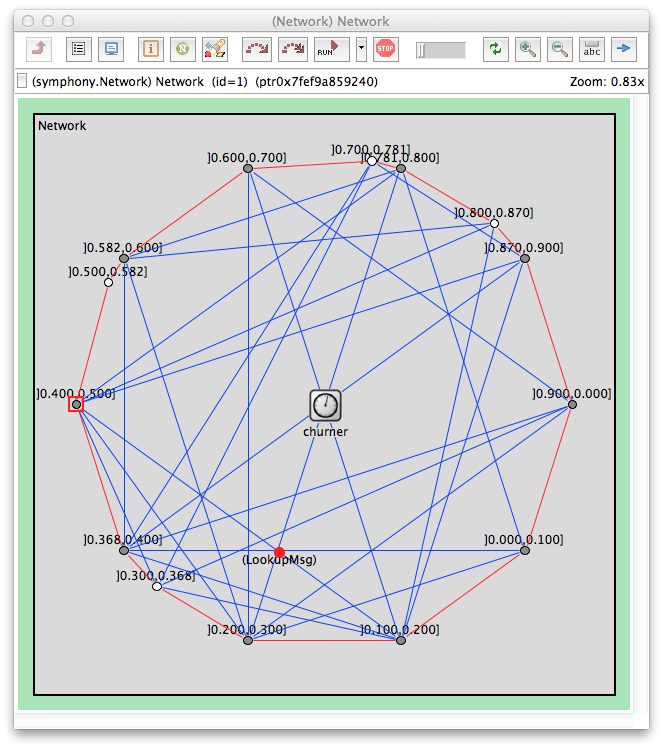
\includegraphics[scale=0.32]{imgs/screenshot.png}
\caption{Una screenshot della simulazione. Possiamo notare i long link colorati di blu ed i short link colorati di rosso. I nodi più scuri sono i peer statici, mentre quelli più chiari sono quelli dinamici. Ogni peer ha poi una label che indica il range di valori che vengono amministrati da tale nodo.}
\end{center}
\end{figure}

\subsection{Il simulatore di Symphony}

La simulazione è costituita da una rete, contenente una serie di peer collegati tra loro attraverso dei canali di comunicazione. Inoltre il simulatore comprende un'entità speciale, diversa dal peer, chiamata \emph{Churner}, che gestisce l'entrata e l'uscita dei peer secondo due parametri configurabili relativi rispettivamente alla \emph{frequenza di entrata} (\texttt{join\_freq}) e alla \emph{frequenza di uscita} dei peer (\texttt{leave\_freq}). Questa è la componente che permette di simulare il churn e quindi di misurare conseguentemente la stabilità del protocollo.

La rete viene configurata mediante il numero di peer presenti all'interno della simulazione. In tutte le simulazioni, invece, i canali di comunicazione della rete sono stati settati con delay di 100ms e bandwith di 10Mbps.

Il peer rappresenta un generico nodo della rete. Esso mantiene alcune informazioni necessarie:
\begin{itemize}
	\item ~Un id $id_i \in [0,1)$, che identifica univocamente il peer $p_i$ all'interno della rete di overlay Symphony.
	\item ~Un canale di comunicazione verso il nodo precedente, ed un altro verso il successivo. Questi costituiscono gli \textit{short link} di Symphony.
	\item ~Un array di canali di comunicazione verso peer arbitrari della rete. Questi costituiscono i \textit{long link} di Symphony.
\end{itemize}

Inoltre ogni peer può contare su una serie di parametri identici per ogni peer, che delineano in modo parametrico il loro comportamento finale:
\begin{itemize}
	\item ~Il parametro \textit{k}, che costituisce il numero di long link che il peer deve provare a instaurare.
	\item ~Un parametro per stabilire il numero di tentativi che il peer è disposto a fare per costruire i long link. Ciò viene accuratamente descritto nell'articolo originale di Symphony.
	\item ~Un parametro che indica se il peer utilizza il protocollo di \emph{relinking} o meno.
\end{itemize}

Inoltre, ai fini della simulazione del churn, i peer sono suddivisi in due classi distinte: i peer \emph{statici} e i peer \emph{dinamici}. Descriviamo nel seguito le caratteristiche delle due classi di peer.

\subsubsection*{Peer statici}
Un peer statico è un peer che entra nella rete all'inizio della simulazione e non esce più dalla rete. Esso quindi non fa parte dei peer gestiti dal Churner. Ogni peer statico $p_i$ ha un $id_i \in [0,1)$ deterministico uniformemente distribuito nell'anello: se rappresentiamo i peer statici come $\{sp_1, \linebreak[1] sp_2, \linebreak[1] ..., \linebreak[1] sp_n\}$, abbiamo che $id_i = i / n$.

Gli short link dei peer statici vengono definiti direttamente nel file NED. I long link, invece, non possono essere definiti nel file NED a causa del potere espressivo troppo debole del linguaggio NED stesso. Sarebbe infatti possibile costruirne soltanto un'approssimazione dei long link, la quale non garantirebbe l'assenza di conflitti (ad esempio, un long link che collega due nodi già connessi), né tantomeno si garantirebbe la conformità al protocollo Symphony (ad esempio, non si potrebbe implementare il massimo numero di tentativi per la creazione dei long link, che permette di risolvere situazioni di rete satura). Pertanto, i long link vengono creati dagli stessi peer statici all'inizio della simulazione, senza l'utilizzo di messaggi. In questo modo, è necessario attendere un breve periodo, chiamato \textit{periodo di warmup}, prima di poter registrare i dati della simulazioni. In particolare, il Churner deve attendere tale periodo prima di iniziare la fase di churn.

\subsubsection*{Peer dinamici}
I peer dinamici vengono inseriti nella rete solo quando deciso dal Churner. All'inizio, quindi, essi si trovano all'esterno della rete di overlay, e non stabiliscono né short link né long link.

Un peer dinamico rimane quindi in disparte fino a quando il Churner, attraverso un messaggio, non gli chiede di entrare a far parte della rete. A quel punto, come stabilito da Symphony, questi calcola il suo id $x$ e individua l'attuale manager di $x$ attraverso un lookup, contattando un nodo della rete noto a priori (un nodo casuale tra quelli statici, scelta che garantisce uniformità nel carico in questa prima fase).

Un peer dinamico, dopo essere entrato all'interno della rete di overlay, rimane al suo interno fintantoché il Churner non gli chiede di uscire. A quel punto il peer non deve far altro che eliminare tutti i collegamenti, ripristinando la topologia, e ritornare nella sua fase iniziale, attendendo nuovamente di poter rientrare. 

Quando il peer dinamico si trova fuori dalla rete, può ricevere comunque dei messaggi (ad esempio, quelli che gli sono stati mandati poco prima la sua uscita, ancora in transito al momento dell'uscita). Tali messaggi verranno scartati dal peer e rimandati al mittente, in modo da simulare fedelmente ciò che accadrebbe nella realtà (si pensi ai tempi di attesa nel caso in cui provassimo a contattare un nodo esistente che non vuole accettare una richiesta di connessione). In tal modo, il mittente potrà re-inviare il messaggio al peer più appropriato (si pensi ad esempio al lookup).

\subsubsection*{Il Churner}
Il Churner è l'entità esterna alla rete di overlay che gestisce il churn. Le sue funzionalità base sono: (1) comunicare ogni \texttt{join\_freq} secondi ad un peer dinamico scelto casualmente tra quelli all'esterno della rete di entrare e (2) comunicare ogni \texttt{leave\_freq} secondi ad un peer dinamico scelto casualmente tra quelli già entrati nella rete di uscire. Il Churner quindi partiziona l'insieme dei peer dinamici in quattro sottoinsiemi: i peer esterni alla rete e che non stanno entrando, i peer esterni cui è stato chiesto di entrare e che stanno completando le operazioni di join, i peer entrati nella rete e che non stanno per uscire, e infine i peer dentro la rete cui è stato chiesto di uscire e che stanno completando le operazioni di uscita.

La scelta di gestire il churn attraverso questa entità esterna è motivata dal fatto che lasciare che siano i peer stessi a gestire le loro entrate e uscite richiederebbe l'implementazione di una complessa coordinazione tra di loro. Il Churner offre un controllo del churn più flessibile e semplice.


\subsection{Il livello di astrazione e i messaggi}

%simulazione della sola rete di overlay
Una prima osservazione riguarda la topologia della rete simulata. Come viene solitamente fatto nelle simulazioni riguardanti reti di overlay peer-to-peer, la simulazione astrae da dettagli relativi alla reale topologia fisica dei nodi, ovvero la loro effettiva distribuzione nel territorio. Inoltre, vengono ignorati tutti i dettagli relativi ai protocolli di comunicazione di più basso livello (ad esempio TCP/IP). La simulazione presenta solamente un delay dei canali di comunicazione di 100ms e un bandwith di 10Mbps, che stimiamo essere una buona approssimazione di un tipico canale di comunicazione su Internet.

%La simulazione, come abbiamo precedentemente visto, è composta dai vari peer, collegati tra di loro mediante gli short link ed i long link. Una prima osservazione sul livello di astrazione è pertanto quella che riguarda la topologia della rete che collega tali peer. Nella realtà, ogni peer fa parte della rete reale di Internet, che è differente dalla rete di overlay logica creata da Symphony. Nella nostra simulazione, viene rappresentata solamente quest'ultima, dove ogni link (sia short che long) ha un delay di 100ms ed un bandwith di 10Mbps, che stimiamo essere una buona approssimazione di un usuale canale di comunicazione logico, che colleghi due peer presenti sulla rete di Internet.

%come abbiamo risolto gli accessi a sezioni critiche
In una reale implementazione del protocollo, i peer che entrano ed escono dalla rete hanno bisogno di meccanismi di accesso in sezione critica distribuiti, per non creare delle incoerenze che potrebbero intaccare negativamente la struttura della rete di overlay. Tali meccanismi sono a volte complessi da implementare e non sono oggetto del nostro studio. È stato pertanto sfruttato il fatto che il simulatore genera eventi discreti mai gestiti in concorrenza tra loro (il simulatore non è parallelo). Tutte le manipolazioni della topologia vengono fatte dal peer interessato, in un solo metodo, compiendo pertanto azioni atomiche. Per esempio, si consideri il caso di un peer $p$ che vuole entrare nella rete con un id $x$. Nella nostra simulazione, è l'attuale manager di $x$ colui il quale modifica gli short link per far entrare $p$ all'interno della rete, diversamente da come dovrebbe avvenire in una reale implementazione del protocollo.

%conoscenza del vicinato
Si assume inoltre che ogni peer abbia conoscenza dei peer che compongono il proprio vicinato (due nodi per gli short link e meno di sei per i long link). Questa è un'assunzione realistica, comunemente utilizzata nei reali sistemi peer-to-peer. In questo modo ogni peer conosce con esattezza il sotto-intervallo da esso gestito, nonché quale dei propri vicini gestisce l'id più vicino ad una certa $x$, nel momento in cui è necessario un foward per il protocollo di routing. In una reale implementazione queste due considerazioni continuerebbero a valere, rendendo questi aspetti fedelmente emulati.
%Ogni peer conosce pertanto l'id di ogni suo vicino, recuperato al momento della creazione del link che li ha connessi. Lo stesso non si può dire per gli id gestiti da un peer vicino, poiché in questo caso tale informazione cambia continuamente. 

%che id gestisco? qual'è il peer vicino migliore per forwardare un messaggio?
%Ciò è necessario per chiarire due due cose molto importanti. La prima è sapere quali sono gli id gestiti dal proprio peer: tale informazione viene ottenuta senza l'invio di nessun messaggio, considerando il proprio id e quello del peer precedente. La seconda è sapere a chi dobbiamo fare il forward di un messaggio di lookup che richiede di cercare il manager dell'id $x$. Anche in questo caso, senza mandare messaggi, possiamo semplicemente controllare gli id di ogni peer vicino, e fare il forward al peer con l'id più vicino ad $x$, rispettando le specifiche del Routing Protocol descritto da Symphony. In una reale implementazione queste due considerazioni continuerebbero a valere, rendendo questi aspetti fedelmente emulati.

\subsubsection*{Messaggi}

Ogni peer può mandare e ricevere diversi messaggi:
\begin{itemize}
	\item ~\texttt{LookupMsg}: è il messaggio di lookup. Tale messaggio può essere utilizzato per tre motivi diversi: per cercare il manager di un id quando viene fatto un join, per cercare il manager di un id per poter creare un long link, oppure per un lookup generico che simula la ricerca di un file all'interno della rete.
	\item ~\texttt{LookupResponseMsg}: è la risposta ad un lookup, che trasporta al suo interno l'identificatore del manager. In questo modo il peer che ha fatto la richiesta può compiere un'azione opportuna.
	\item ~\texttt{NEstimationMsg}: è il messaggio che viene spedito per aggiornare la stima del numero di peer presenti all'interno della rete, come previsto dal protocollo di Symphony.
\end{itemize}

%id nei messaggi di lookup, coda dei messaggi di uscita
Ogni richiesta di lookup emessa da un determinato peer viene identificata con un id crescente. Anche nel caso in cui un peer uscisse e rientrasse nella rete, tale id è garantito essere distinto.
Ogni peer mantiene inoltre la coda dei lookup richiesti, associando ad ognuno di essi la corrispettiva procedura di callback da eseguire al termine del lookup.
%Ogni risposta ad un lookup (cioè, un \texttt{LookupResponseMsg}) mantiene al suo interno questi id, permettendo al peer, grazie alla coda, di identificare e continuare a svolgere la procedura che aveva richiesto il lookup (il messaggio viene ignorato se non si dovesse trovare nella coda una corrispondenza).
Tale coda viene svuotata al momento dell'uscita del peer dalla rete, permettendo di ignorare le risposte a lookup inviati in una precedente reincarnazione del peer.

%join
%Per utilizzare i messaggi di lookup in modo da effettuare un join, il peer segna in maniera opportuna un campo all'interno del messaggio stesso, in modo da distinguerlo. Così facendo, il manager dell'id, invece di rispondere solamente a tale lookup, può manipolare la topologia della rete di overlay, in modo da far entrare il peer al suo interno. Le operazioni di join non possono infatti essere fatte dal peer stesso, poiché, durante il tempo trascorso per la ricezione della risposta del lookup, il manager può non gestire più l'id che gli era stato richiesto, generando conflitti che perturberebbero la topologia della rete di overlay. Il join, compiendo un'azione atomica per manipolare la topologia, utilizza pertanto un numero di messaggi che nella realtà sarebbe più alto. 

Nel caso in cui un lookup sia stato chiesto per effettuare un join con id $x$ (ovvero, il primo lookup chiesto da ogni peer), il messaggio di lookup contiene un campo opportuno che segnala al manager di $x$ di effettuare le operazioni di creazione degli short link. Ciò ha l'unico scopo di evitare, come discusso in precedenza, l'implementazione di una sezione critica distribuita non oggetto del presente studio.

%leave
L'operazione dei leave  viene fatta dal peer in maniera atomica, anche qui sfruttando il concetto discusso precedentemente, in modo da evitare gestione complessa della concorrenza. Come nel caso del join, il numero di messaggi inviati è minore di quello che sarebbe necessario in una reale implementazione del protocollo.




\section{Risultati sperimentali} \label{risultati}
Riportiamo in questa Sezione i risultati sperimentali sulla stabilità del protocollo Symphony, derivanti dalle simulazioni realizzate per mezzo del nostro simulatore.

\subsection{Validazione del simulatore}

\begin{figure}	
\minipage{0.50\textwidth}
\centering
	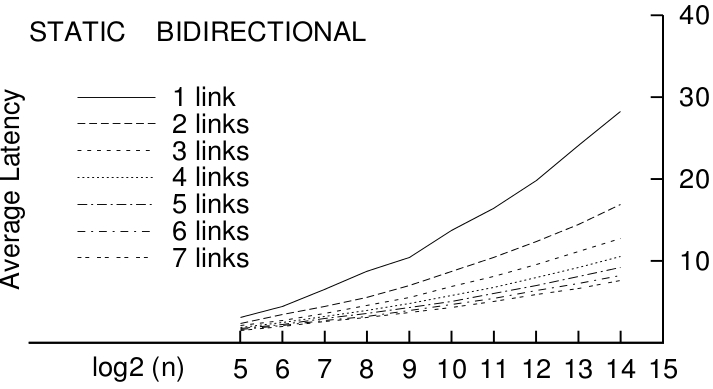
\includegraphics[scale=.31]{imgs/join-reale.jpg}
\endminipage\hfill
\minipage{0.50\textwidth}
\centering
	\includegraphics[scale=.31, angle=-90]{imgs/join_cost.eps}
\endminipage\hfill
\caption{Validazione del simulatore: a sinistra le latenze medie registrate nel paper originale, a destra quelle registrate utilizzando il nostro simulatore. In entrambi i casi, i tempi di latenza sono polilogaritmici.}
\label{img:join-cost}
\end{figure}

Il primo esperimento che riportiamo è atto a supportare la validazione del simulatore realizzato. La validazione effettuata riguarda il protocollo di routing. Come nel paper originale, il numero dei peer nella rete viene fatto variare da $2^5$ a $2^{14}$ e vengono misurati gli hop medi per lookup. Nel paper vengono fatti esperimenti variando $k$, il numero massimo di long link, mentre nel nostro caso $k$ è stato tenuto fisso a $5$ [-------------------------- METTERE VALORE CORRETTO ----------------]. Il nostro simulatore inoltre utilizza solo routing bidirezionale.

In Figura~\ref{img:join-cost} mettiamo a paragone i risultati delle simulazioni del paper originale (a sinistra) con quelli del nostro simulatore (a destra). Ogni punto della Figura relativa al nostro simulatore è il risultato della media di 10 run di simulazione, ognuno dei quali ha registrato il numero di hop di 100 lookup. Dalla Figura è evidente come l'andamento della curva relativa alla latenza media dei lookup sia identico nei due simulatori, ovvero polilogaritmico nel numero dei peer presenti nella rete. Questo risultato valida il nostro protocollo di routing simulato per mezzo di Omnet++, come precedentemente descritto. La Figura mostra anche come gli intervalli di confidenza, misurati al 95\% con distribuzione t-student, siano sufficientemente stretti intorno alla media [----------- CONTROLLARE QUI ----------------], il che contribuisce a validarne i risultati.

[--------------TODO: COME DISCUTERE LA DIFFERENZA TRA 30 e 60??? ---------------]




\subsection{Stabilità senza re-linking}
% Al variare di frequenza
% Al variare del numero di peer che entrano nello stesso tempo: discutere della velocità di crescita di N rispetto alla velocità di decrescita di H
Al fine di misurare la stabilità del protocollo Symphony secondo le definizioni di stabilità presentate in Sezione~\ref{stabilita}, sono stati svolti due test. Nel primo test viene calcolato il valore di $stability(H,N)$ al variare della frequenza del churn. Nel secondo test viene calcolato lo stesso valore al variare del numero di peer che stanno entrando contemporaneamente nella rete. I due test, sebbene possano sembrare simili, presentano una differenza importante, ed evidenziano una caratteristica fondamentale della nostra definizione di stabilità e del protocollo Symphony.

Nel primo test la rete viene stressata controllando la frequenza a cui viene chiesto ai peer di entrare e uscire dalla rete. Il Churner, come descritto precedentemente, chiede ad un peer di entrare ogni \texttt{join\_freq} secondi, e ad un altro di uscire ogni \texttt{leave\_freq} secondi. Nel momento in cui ad un peer viene chiesto di entrare, esso comincia la prima procedura di lookup del manager relativo al suo nuovo id. Solo dopo averlo trovato, il peer si unisce alla rete, inizialmente utilizzando soltanto due short link, in modo da chiudere l'anello. In quel momento, comincia la sua procedura di creazione dei long link, la quale terminerà solo dopo averne creato un numero sufficiente, secondo le specifiche di Symphony.

È proprio durante questa fase che la rete può mostrare potenziali segni di instabilità. Se il peer appena entrato è l'unico con soli short link, l'effetto della mancanza dei suoi long link non sarà particolarmente evidente nella totalità delle misurazioni. Di contro, se vi è un numero considerevole di peer in fase di creazione di long link, il numero degli hop per lookup in media può aumentare considerevolmente. Nel caso pessimo, come discusso in precedenza, tale numero è $O(n)$, quando il routing del lookup incontra soltanto peer senza long link instaurati.

\subsubsection{Stabilità al variare della frequenza dei join}

\begin{figure}	
\minipage{0.33\textwidth}
\centering
	\includegraphics[scale=.22, angle=-90]{imgs/norelink-freq-hops.eps}
\endminipage\hfill
\minipage{0.33\textwidth}
\centering
	\includegraphics[scale=.22, angle=-90]{imgs/norelink-freq-time.eps}
\endminipage\hfill
\minipage{0.33\textwidth}
\centering
	\includegraphics[scale=.22, angle=-90]{imgs/norelink-freq-stability.eps}
\endminipage\hfill
\caption{*********************}
\label{img:stabilita}
\end{figure}

In Figura~\ref{img:stabilita} mostriamo i risultati del primo test, in cui variamo la frequenza dei join in modo crescente.

In tutte le simulazioni sono stati utilizzati 32 peer statici (ovvero, entrati prima dell'inizio delle registrazioni e mai usciti dalla rete) e 8 peer dinamici. Gli 8 peer dinamici sono stati fatti entrare e uscire 2048 volte. In questo modo è stato possibile aggregare molti valori registrati dallo stesso peer. Una volta che uno di questi peer è entrato e ha completato tutta la sua fase di creazione dei long link, il Churner gli ha chiesto di uscire dopo 0.1ms. La frequenza di entrata, invece, è stata fatta variare da 1 peer ogni $10^6$ millisecondi ad 1 peer ogni $10^{-8}$ millisecondi. Ogni punto rappresentato nella curva in Figura è il risultato della media di 10 run di simulazione.

In Figura~\ref{img:stabilita}(a) mostriamo la latenza media dei lookup (ovvero, il numero medio degli hop). In Figura~\ref{img:stabilita}(b) mostriamo i tempi medi di lookup, calcolati in secondi. Infine, in Figura~\ref{img:stabilita}(c) mostriamo il valore della stabilità. Ogni punto della curva di stabilità è un valore $stability(H_i,N_i)$, corrispondente all'$i$-esima frequenza di join, tale che $H_i = \{ h_1, h_2, \dots, h_{10} \}$ e $N_i = \{ n_1, n_2, \dots, n_{10} \}$ per 10 run di simulazione nei quali $h_j$ e $n_j$ sono rispettivamente il numero di hop medi e il numero di peer medi misurati al $j$-esimo run.

[----- HOPS E TEMPO UGUALI ----]
[----- STABILITA INVERSAMENTE AL HOP ----]
[----- AUMENTO ESPONENZIALE DEGLI HOP E DIM. DELLA STABILITA. TIP POINT ----]


\subsection{Stabilità con re-linking}
\vspace*{100mm}
% Come prima: mostra che non cambia molto perché relinking non scatta
% Mostra che cambiando alcuni parametri si fa scattare il relinking e le cose peggiorano molto

\subsection{Calcolare $\epsilon^*$ di Symphony}
\vspace*{100mm}



\section{Conclusioni} \label{conclusioni}
\vspace*{100mm}











% Appendix
%\appendix
%\section*{APPENDIX}
%\setcounter{section}{1}



% Bibliography
\bibliographystyle{ACM-Reference-Format-Journals}
\bibliography{bibliografia}

% History dates
%\received{February 2009}{July 2009}{October 2009}




%\elecappendix


%\section{Analysis of Invalid Trials}
%\label{invalid}

%\subsection{Results}




\end{document}
% End of v2-acmlarge-sample.tex (March 2012) - Gerry Murray, ACM
